\documentclass[notes]{beamer}
\usepackage{pgfpages}
%\setbeameroption{show notes on second screen}
\usetheme{Montpellier}
\usepackage{graphicx}
\usepackage{minted}

\title{Code Your Own Website \\ Basic HTML and CSS}
\date{Updated as of: \today}

\begin{document}
\section{Introduction}
\begin{frame}
  \maketitle
  \note{This class is going to cover very basic HTML and CSS and how these design languages are used to build simple webpages. We'll be building a number of examples using the site Neocities which provides free hosting.}
\end{frame}

\begin{frame}{What you're learning}
  \begin{block}{The important pieces}
    \begin{description}
      \item[HTML] \textbf Hyper\textbf Text \textbf Markup \textbf Language
      \item[CSS] \textbf Cascading \textbf Style \textbf Sheets
      \item[JavaScript] A programming language
    \end{description}
  \end{block}
  \note{
    HTML is the like the bones, the architecture, of a webpage. It includes the basic \textit{content} of the webpage: there's a button here, a paragraph there, a link here. HTML by itself leads to very plain looking pages, like the ones we had in the 90s.

    CSS describes how things should look, it's the code that says what colors things should be, how wide columns of text are, and even things like whether pictures should appear square or round like in a frame. 
  }
\end{frame}

\begin{frame}{Why learn it?}
  \begin{block}{}
    \centering
    {\huge Why code a site by hand?}
  \end{block}
  \note{
    There's a lot of services now such as Wix, Wordpress, and Google Sites that are meant to help you build webpages without having to actually understand the code that goes into them.

    I'm not denigrating those services in any way, but there's a few reasons why you might want to know how to write HTML, CSS, and JavaScript yourself.

    First, so that you're not entirely reliant on services such as Google Sites. It's empowering to know how to do something yourself even if you ultimately decide to not do so. You'll at least have had the choice!

    Second, so that you can create something that looks unique and interesting. The problem with site-building services is that they tend to create sites that all look alike. Most wordpress sites, unless very heavily customized, are recognizable as wordpress sites.

    Finally, because it might just be fun. I think there's a pleasure to coding and crafting that can just be for its own sake.
  }
\end{frame}

\begin{frame}{What we'll be using}
  \begin{block}{Neocities}
    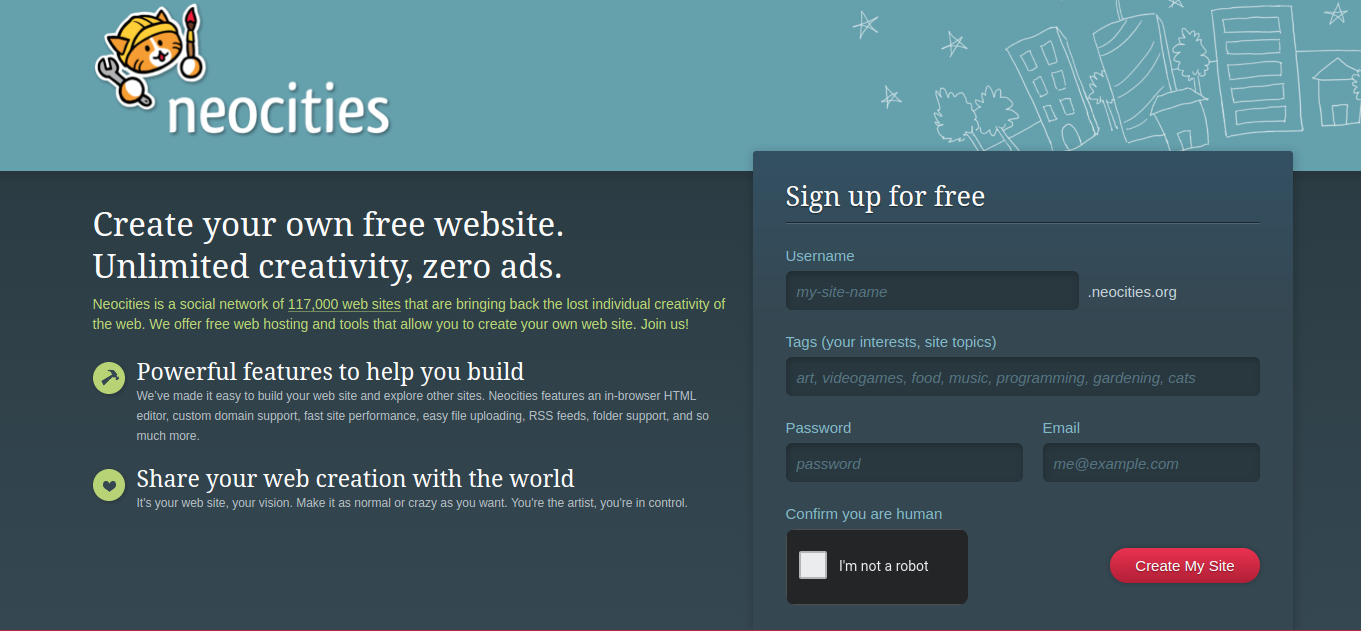
\includegraphics[width=4in]{signup}
  \end{block}
\note{Neocities is a free hosting service that allows you to write all the code for your website. It's a pretty solid product that I highly recommend. There's a password provided for an in-class account that we'll be sharing, but if you want to continue working on your own you can sign up for your own account.}
\end{frame}
\section{Basic HTML}
\begin{frame}[fragile]{What does HTML look like?}
  \begin{minted}[fontsize=\footnotesize]{html}
    <!doctype html>
    <html>
    <body>
    <h1>The heading at the top goes in the h1 tags</h1>

    <p> This is a paragraph
    and it doesn't matter
    how I put    
    linebreaks, only that I put it within the tags</p>
    <ol>
      <li> This is going to look like</li>
      <li> A numbered list</li>
    </ol>
    <button>Press me!</button>
    <p> that button is for show since there's no code running it</p>
    </body>
    </html>
  \end{minted}
  \note{You'll notice that there's a pattern here of these <..> </..> pairs, like the <h1> </h1> and the <p> </p> pairs. These nested pairs are called \textit{tags} and these tags are how you say ``everything between here and here is a part of this''. So, for example, everything between <h1> and </h1> is a part of the \textit{heading}. Everything between a <p> and </p> pair \textit{is} a paragraph.}
\end{frame}

\begin{frame}{How does it look in the browser?}
  \includegraphics[width=4in]{AltHtmlExample}
  \note{You can see in this screenshot that putting in linebreaks didn't change the way that first paragraph looked. HTML doesn't care about how you space things, only the tags you use. You could have put this entire file on one ugly line and the browser would have read it exactly the same way!}
\end{frame}

\begin{frame}[fragile]{Trying it out}
  \begin{columns}
    \begin{column}{0.35\columnwidth}
      \begin{block}{Instructions}
        \begin{enumerate}
          \item Go to the class neocities page
          \item Choose to make a new file, call it \texttt{AAAex.html}
          \item Delete the starter text
          \item Type the text in the right hand column, and hit \texttt{view}
        \end{enumerate}
      \end{block}
    \end{column}
    \begin{column}{0.65\columnwidth}
      \begin{block}{Type this verbatim}
        \begin{minted}[fontsize=\footnotesize]{html}
        <!doctype html>

        <html>
        <body>
          <h1>This is a heading</h1>
          <p>Here is a paragraph. 
          It has a <q>quote</q> in it.</p>
          <ol>
            <li>here's a list</li>
            <li>it has elements</li>
          </ol>
          <button>Pointless</button>  
        </body>
        </html>
      \end{minted}
      \end{block}
    \end{column}
  \end{columns}
\end{frame}

\begin{frame}{Mozilla Developer Network}
  \begin{block}{\url{https://developer.mozilla.org/en-US/}}
    \includegraphics[width=4in]{UpdatedMDN}
  \end{block}
  \note{The Mozilla Developer Network is a great place to continue learning about web development. They have a lot of tutorials and reference guides that are all freely available. Go ahead and navigate to this page and take a few minutes to look around before we go onto the next exercise.}
\end{frame}

\begin{frame}{Experimenting with tags}
  \begin{block}{}
    Now take a few minutes and play around with the example you already wrote and try adding different tags and seeing what it looks like. 
    Some things you might want to try
    \begin{itemize}
      \item <ul>
      \item <input>
      \item <h2>--<h6>
      \item <blockquote>
    \end{itemize}
  \end{block}
  \note{You can also look up more documentation at the Mozilla Developer network that we've discussed. You might also want to try lookinag at the documenation for the <input> tag because it actually has a bunch of different forms that let you define everything from text fields to date entry with a calendar: \url{https://developer.mozilla.org/en-US/docs/Web/HTML/Element/input}}
\end{frame}

\begin{frame}[fragile]{Links}
      \begin{block}{}
        \begin{minted}[fontsize=\scriptsize]{html}
          <a href="http://multcolib.org">Multnomah County Library System</a>
        \end{minted}
      \end{block}
      \begin{block}{}
        \centering
        \includegraphics[width=2in]{LinkExample}
      \end{block}
      \note{All links are of the form <a href="[insert web address here]">[Text of the link]</a> where you replace the square brackets and everything inside it with the URL and the text that should \textit{appear} for the link. This is our first example of an \textit{attribute} in HTML, which is a way to give extra information that changes what a tag does. If you played around with the <input> tag above you might have seen that there's an attribute that changes the form of the input. With the <a> tag, the attribute sets the website that the link goes to.

        If you're wondering, the ``a'' in <a> stands for \textit{anchor}. The <a> tag can actually be used for things other than links to other web pages, but that's probably what it's used for the most.}
\end{frame}

\begin{frame}[fragile]{Images}
  \begin{block}{}
      \begin{minted}{html}
        <image src="http://bit.ly/2viv8Uh">
      \end{minted}
  \end{block}
  \begin{block}{}
    \centering
    \includegraphics[width=2.5in]{silkie}
  \end{block}
  \note{Including images involves another \textit{attribute}, this time one that defines the ``source'' of the image. Images are also one of only a couple of tags that don't have a closing tag, only an opening tag!

  At this point, you might want to even try grabbing an image or two and 

  }
\end{frame}

\begin{frame}{Try adding images and links!}
  \begin{block}{}
    Try adding links and images to the page you've been working on!
  \end{block}
\end{frame}

\section{Basic CSS}
\begin{frame}[fragile]{First example}
  \begin{minted}{html}
    <html>
      <head>
        <style>
          p {
            color: red;
          }
        </style>
      </head>
      <body>
        <h1>The heading</h1>
        <p>The text in a paragraph</p>
        <p>This is another paragraph</p>
      </body>
    </html>
  \end{minted}
  \note{CSS code is a separate language from HTML that affects how your HTML looks. CSS is one of the main things that makes websites today look different than they did in the 90s, when everything was very simplistic and a bit ugly. The above code changes the color of the text in every paragraph (<p> tag) to red.

    You can include the CSS code directly into the HTML file by putting <style> tags inside the <head> tags, which comes before the <body>.

    Inside the <style> tags you can write CSS code that will automatically be loaded and affect the page.
  }
\end{frame}

\begin{frame}{What it looks like}
  \includegraphics[width=1.5in]{FirstCSSExample}
\end{frame}

\begin{frame}[fragile]{Selecting by tag}
  \begin{minted}[fontsize=\tiny]{html}
<html>
  <head>
    <style>
      p {
        width: 100px;
        color: red;
        font-weight: bold;
      }
      ol {
        list-style: lower-greek;
      }
    </style>
  </head>
  <body>
    <p>Here's some text in a paragraph.
      I'm going to try and type enough
      that it wraps around to show how
      narrow the paragraph is forced to be.</p>

    <ol>
      <li>Here's an item</li>
      <li>Here's another item</li>
    </ol>
  </body>
</html>
  \end{minted}
  \note{As we saw up above, we can select all elements with a particular tag and style them with CSS code. In this case we're making the paragraphs one hundred pixels wide, bold, and with red text. We're also changing all numbered lists to count in lowercase greek letters instead of numerals.

  With CSS just a few lines of code can make a pretty big difference to the overall look of the site.}
\end{frame}

\begin{frame}{What it creates}
  \includegraphics[width=2in]{TagSelectionExample}
\end{frame}

\begin{frame}[fragile]{Selecting by class}
  \begin{minted}[fontsize=\tiny]{html}
<html>
  <head>
    <style>
      .pullquote {
        font-style: italic;
        border-top: solid;
        border-bottom: solid;
        font-size: 16pt;
        width: 150px;
      }
    </style>
  </head>
  <body>
    <p>This is some text that's normal</p>
    <p class="pullquote">They're good dogs, Brent</p>
    <p>So one of the best internet memes comes
      from the twitter account @dog_rates,
      which gives surreal numeric ratings to dogs.
    </p>
    <p>
      The owner of the account once got into an
      in-character argument with a man named Brant...
    </p>
  </body>
</html>    
\end{minted}

 \note{A class is a special attribute that works with CSS. You can then choose to style \textit{everything} with that class the same way. In this case we've made a little class that we can use to create stylized pullquotes out of a normal paragraph. Any paragraph you give the class pullquote to will then be style \textit{very} differently. In order to select a class in the CSS, you want to prepend a . to the class name. So even though our pullquote class is just called \texttt{pullquote}, you reference it in CSS code as \texttt{.pullquote}}
\end{frame}

\begin{frame}{What it looks like}
  \includegraphics[width=4in]{ClassSelectionExample}
\end{frame}


\begin{frame}{Let's try it}
  \begin{block}{}
    Now try out what you've seen and play with the CSS of your file
  \end{block}
\end{frame}

\section{A taste of JavaScript}
\begin{frame}[fragile]{Our first JavaScript example}
  \begin{minted}[fontsize=\scriptsize]{html}
<html>
  <head>
  <script>
window.onload = function () {

var input = document.getElementById("input");
var but = document.getElementById("button");

but.addEventListener("click", function () {
    alert(input.value);
});

}
  </script>
  </head>
  <body>
    <input id="input" value="stuff"/>
    <button id="button">Press me</button>
  </body>
</html>
  \end{minted}
  \note{JavaScript is a programming language that runs in the browser. It allows us to add dynamics to the webpage, making web pages interactive instead of static. This is a tiny example that just extracts the text out of the input and creates a pop-up alert with that text inside.}
\end{frame}

\section{Where to go next}
\begin{frame}{What to try now}
  \begin{block}{}
    \begin{itemize}
      \item Make your own Neocities account
      \item Read through MDN's tutorials
      \item Take the sequel web development class
    \end{itemize}
  \end{block}
\end{frame}

\end{document}